\documentclass{article}\usepackage[]{graphicx}\usepackage[]{color}
%% maxwidth is the original width if it is less than linewidth
%% otherwise use linewidth (to make sure the graphics do not exceed the margin)
\makeatletter
\def\maxwidth{ %
  \ifdim\Gin@nat@width>\linewidth
    \linewidth
  \else
    \Gin@nat@width
  \fi
}
\makeatother

\definecolor{fgcolor}{rgb}{0.345, 0.345, 0.345}
\newcommand{\hlnum}[1]{\textcolor[rgb]{0.686,0.059,0.569}{#1}}%
\newcommand{\hlstr}[1]{\textcolor[rgb]{0.192,0.494,0.8}{#1}}%
\newcommand{\hlcom}[1]{\textcolor[rgb]{0.678,0.584,0.686}{\textit{#1}}}%
\newcommand{\hlopt}[1]{\textcolor[rgb]{0,0,0}{#1}}%
\newcommand{\hlstd}[1]{\textcolor[rgb]{0.345,0.345,0.345}{#1}}%
\newcommand{\hlkwa}[1]{\textcolor[rgb]{0.161,0.373,0.58}{\textbf{#1}}}%
\newcommand{\hlkwb}[1]{\textcolor[rgb]{0.69,0.353,0.396}{#1}}%
\newcommand{\hlkwc}[1]{\textcolor[rgb]{0.333,0.667,0.333}{#1}}%
\newcommand{\hlkwd}[1]{\textcolor[rgb]{0.737,0.353,0.396}{\textbf{#1}}}%
\let\hlipl\hlkwb

\usepackage{framed}
\makeatletter
\newenvironment{kframe}{%
 \def\at@end@of@kframe{}%
 \ifinner\ifhmode%
  \def\at@end@of@kframe{\end{minipage}}%
  \begin{minipage}{\columnwidth}%
 \fi\fi%
 \def\FrameCommand##1{\hskip\@totalleftmargin \hskip-\fboxsep
 \colorbox{shadecolor}{##1}\hskip-\fboxsep
     % There is no \\@totalrightmargin, so:
     \hskip-\linewidth \hskip-\@totalleftmargin \hskip\columnwidth}%
 \MakeFramed {\advance\hsize-\width
   \@totalleftmargin\z@ \linewidth\hsize
   \@setminipage}}%
 {\par\unskip\endMakeFramed%
 \at@end@of@kframe}
\makeatother

\definecolor{shadecolor}{rgb}{.97, .97, .97}
\definecolor{messagecolor}{rgb}{0, 0, 0}
\definecolor{warningcolor}{rgb}{1, 0, 1}
\definecolor{errorcolor}{rgb}{1, 0, 0}
\newenvironment{knitrout}{}{} % an empty environment to be redefined in TeX

\usepackage{alltt}
\usepackage{amscd, amssymb, amsmath, verbatim, setspace}
\usepackage[left=1.0in, right=1.0in, top=1.0in, bottom=1.0in]{geometry}
\usepackage{mathrsfs}
\usepackage{listings}


\IfFileExists{upquote.sty}{\usepackage{upquote}}{}
\begin{document}
\begin{flushright}
Arif Ali\\
Math 611 Stochastic Simulation\\
Sept 22, 2016\\
\end{flushright}

\begin{center}
\LARGE\textbf{Homework 3}
  \end{center}
\section*{Exercise 1}
Since $Area_{square}=1$, $Area_{circle}=\frac{\pi}{2^2}=\frac{\pi}{4}$ as stated in the exercise. Therefore the number of points that are expected in the circle is $\frac{\pi/4}{1}= \pi/4$ Given that the orgin of the circle is at $(1/2,1/2)$ with a radius of $r=1/2$, the circle equation is $(x-\frac{1}{2})^2+(y-\frac{1}{2})^2=\frac{1}{4}$, so we should look for points with coordinates such that $(x-\frac{1}{2})^2+(y-\frac{1}{2})^2<\frac{1}{4}$. I assume that the circumference doesn't count as in the circle.
\begin{knitrout}
\definecolor{shadecolor}{rgb}{0.969, 0.969, 0.969}\color{fgcolor}\begin{kframe}
\begin{alltt}
\hlstd{points_in_circle} \hlkwb{=} \hlkwa{function}\hlstd{(}\hlkwc{z}\hlstd{)\{}
  \hlstd{points}\hlkwb{=} \hlkwd{data.frame}\hlstd{(}\hlkwc{x} \hlstd{=} \hlkwd{runif}\hlstd{(}\hlnum{1e3}\hlstd{),} \hlkwc{y} \hlstd{=} \hlkwd{runif}\hlstd{(}\hlnum{1e3}\hlstd{))}
  \hlkwd{mean}\hlstd{((points}\hlopt{$}\hlstd{x}\hlopt{-}\hlnum{1}\hlopt{/}\hlnum{2}\hlstd{)}\hlopt{^}\hlnum{2}\hlopt{+}\hlstd{(points}\hlopt{$}\hlstd{y}\hlopt{-}\hlnum{1}\hlopt{/}\hlnum{2}\hlstd{)}\hlopt{^}\hlnum{2}\hlopt{<}\hlnum{1}\hlopt{/}\hlnum{4}\hlstd{)}
\hlstd{\}}
\hlstd{estimates_of_points_in_circle} \hlkwb{=} \hlkwd{sapply}\hlstd{(}\hlnum{1}\hlopt{:}\hlnum{1e3}\hlstd{, points_in_circle)}
\hlkwd{mean}\hlstd{(estimates_of_points_in_circle)}
\end{alltt}
\begin{verbatim}
## [1] 0.785465
\end{verbatim}
\begin{alltt}
\hlkwd{var}\hlstd{(estimates_of_points_in_circle)}
\end{alltt}
\begin{verbatim}
## [1] 0.0001660909
\end{verbatim}
\begin{alltt}
\hlkwd{hist}\hlstd{(estimates_of_points_in_circle)}
\end{alltt}
\end{kframe}
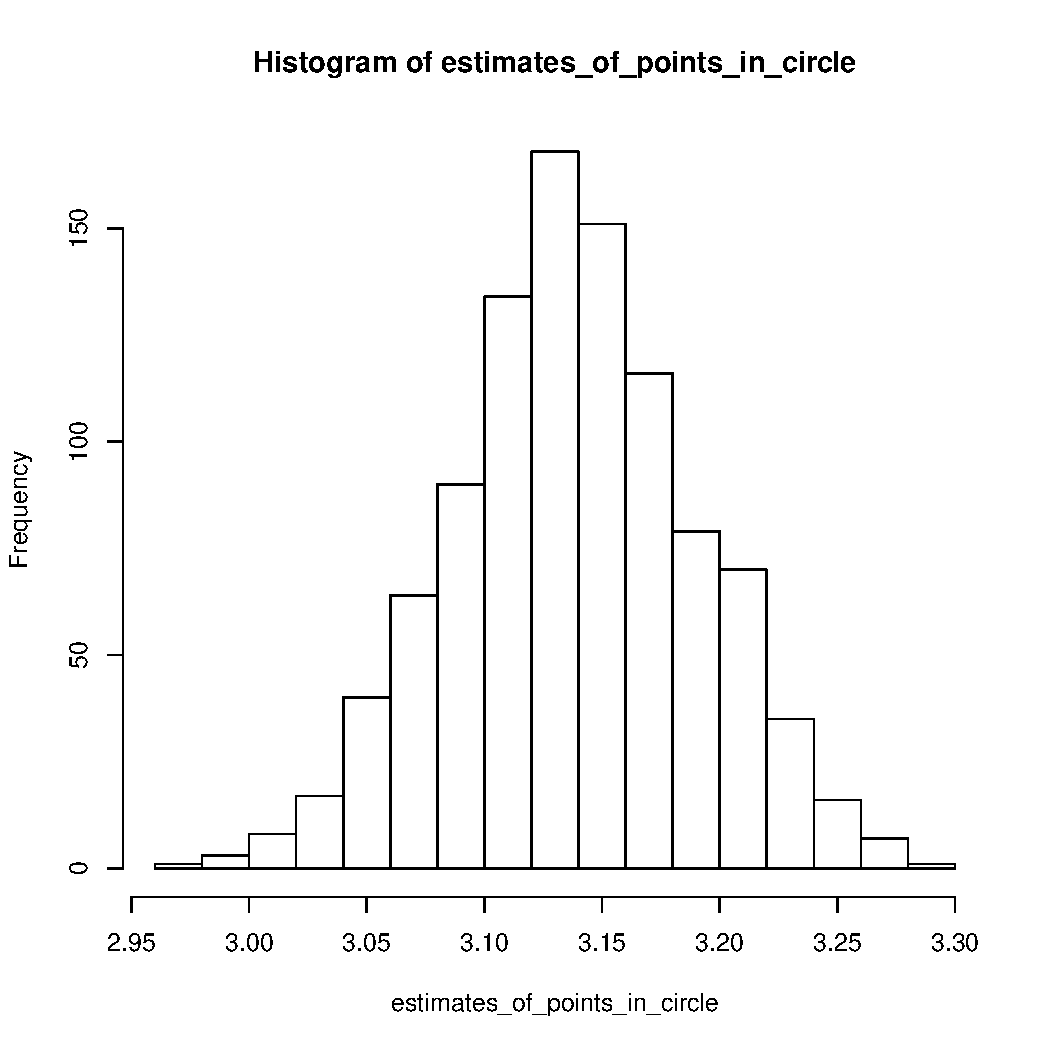
\includegraphics[width=0.60\linewidth]{figure/unnamed-chunk-2-1} 

\end{knitrout}
Based on the estimated mean and the variance, the fixed range is very close to the expected fraction.   
\section*{Exercise 2}
Please note: I used the methods from "http://math.stackexchange.com/questions/1200443/evaluating-difficult-monte-carlo-integration-in-r" to do monte carlo integration in R
\subsection*{Part A}
\begin{knitrout}
\definecolor{shadecolor}{rgb}{0.969, 0.969, 0.969}\color{fgcolor}\begin{kframe}
\begin{alltt}
\hlstd{f} \hlkwb{=} \hlkwa{function}\hlstd{(}\hlkwc{x}\hlstd{)\{}
  \hlkwd{return}\hlstd{(}\hlkwd{exp}\hlstd{(}\hlopt{-}\hlnum{4}\hlopt{*}\hlstd{x}\hlopt{/}\hlnum{3}\hlstd{)}\hlopt{*}\hlstd{x}\hlopt{^}\hlnum{3}\hlstd{)}
\hlstd{\}}
\hlkwd{curve}\hlstd{(f,} \hlkwc{lwd}\hlstd{=}\hlnum{2}\hlstd{,}\hlkwc{to} \hlstd{=} \hlnum{50}\hlstd{)}
\end{alltt}
\end{kframe}
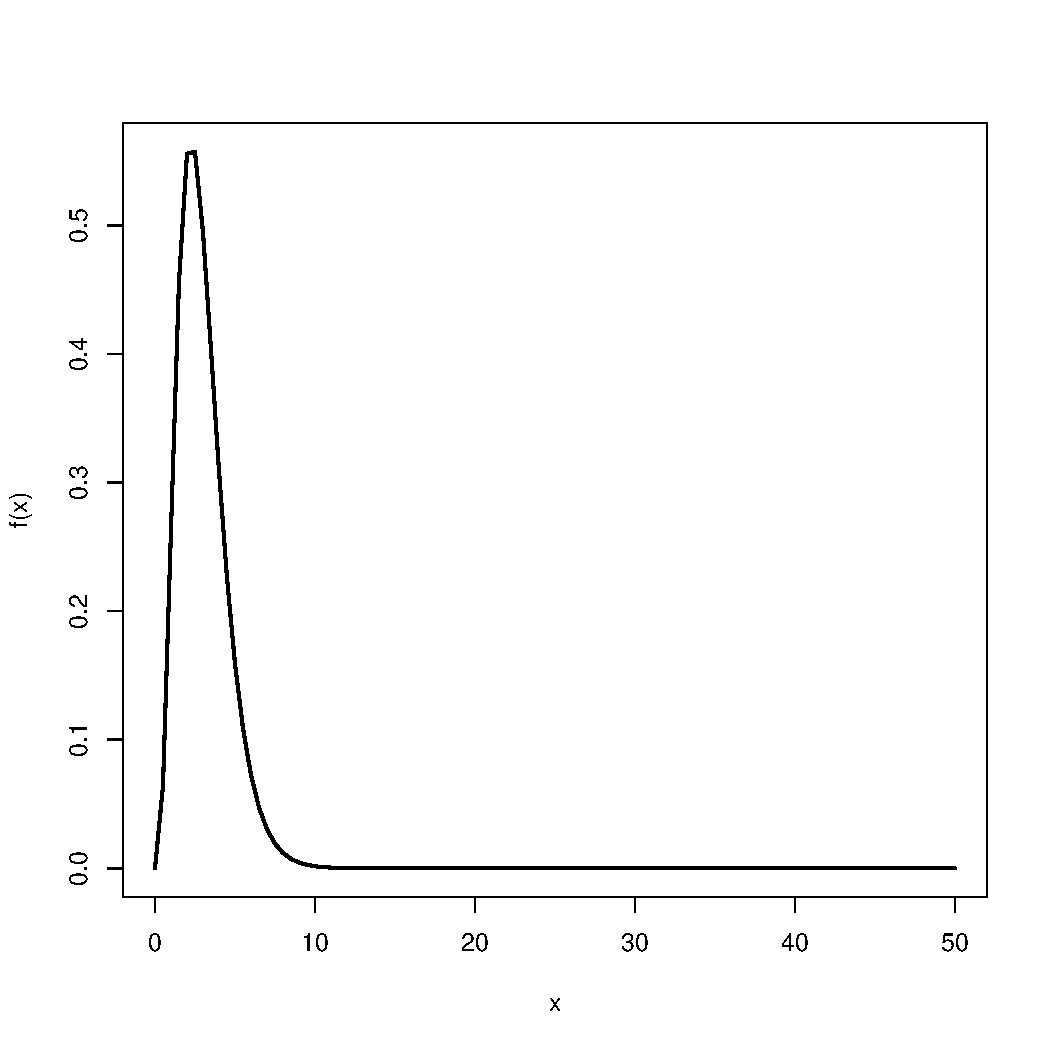
\includegraphics[width=0.60\linewidth]{figure/unnamed-chunk-3-1} 

\end{knitrout}
Based on the graph, it is clear that $f(x)$ converges to 0 close to 10, so using the method described in class, we will do the following:
\begin{knitrout}
\definecolor{shadecolor}{rgb}{0.969, 0.969, 0.969}\color{fgcolor}\begin{kframe}
\begin{alltt}
\hlstd{n} \hlkwb{=} \hlnum{1e4}
\hlstd{a} \hlkwb{=} \hlnum{0}
\hlstd{b} \hlkwb{=} \hlnum{10}
\hlstd{x} \hlkwb{=} \hlkwd{runif}\hlstd{(n, a, b)}
\hlstd{y} \hlkwb{=} \hlkwd{f}\hlstd{(x)}
\hlstd{(b}\hlopt{-}\hlstd{a)}\hlopt{/}\hlstd{n}\hlopt{*}\hlkwd{sum}\hlstd{(y)}
\end{alltt}
\begin{verbatim}
## [1] 1.876069
\end{verbatim}
\end{kframe}
\end{knitrout}
\subsection*{Part B}
\begin{equation}
\begin{split}
\int_{0}^{\infty}e^{\frac{-4x}{3}}x^3\delta x \implies \\
\int_{0}^{\infty}x^3*e^{\frac{-4x}{3}}\delta x \implies \\
\int_{0}^{\infty}x^{4-1}*e^{-\frac{x}{3/4}}\delta x \implies \\
\Gamma(4)*(\frac{3}{4})^4\int_{0}^{\infty}\frac{1}{\Gamma(4)*(\frac{3}{4})^4}*x^{4-1}*e^{-\frac{x}{3/4}}\delta x
\end{split}
\end{equation}
please recognize that $\frac{1}{\Gamma(4)*(\frac{3}{4})^4}*x^{4-1}*e^{\frac{x}{3/4}}\sim gamma(4,3/4)$

$\therefore \Gamma(4)*(\frac{3}{4})^4\int_{0}^{\infty}\frac{1}{\Gamma(4)*(\frac{3}{4})^4}*x^{4-1}*e^{\frac{x}{3/4}}\delta x = \Gamma(4)*(\frac{3}{4})^4 = 1.898$
\section*{Exercise 3}
\begin{knitrout}
\definecolor{shadecolor}{rgb}{0.969, 0.969, 0.969}\color{fgcolor}\begin{kframe}
\begin{alltt}
\hlstd{n} \hlkwb{=} \hlnum{1e4}
\hlstd{a} \hlkwb{=} \hlopt{-}\hlnum{10}
\hlstd{b} \hlkwb{=} \hlnum{10}
\hlstd{x} \hlkwb{=} \hlkwd{runif}\hlstd{(n, a, b)}
\hlstd{y} \hlkwb{=} \hlkwd{exp}\hlstd{(}\hlopt{-}\hlstd{(}\hlkwd{dnorm}\hlstd{(x,} \hlnum{0}\hlstd{,} \hlnum{2}\hlstd{))}\hlopt{^}\hlnum{2}\hlstd{)}
\hlstd{(b}\hlopt{-}\hlstd{a)}\hlopt{/}\hlstd{n}\hlopt{*}\hlkwd{sum}\hlstd{(y)}
\end{alltt}
\begin{verbatim}
## [1] 19.86586
\end{verbatim}
\end{kframe}
\end{knitrout}
\begin{equation}
\begin{split}
E_{f}(h(x)) = \int_{x}\frac{1}{\sqrt{2\pi\sigma^{2}}}e^{-\frac{1}{2\sigma^2}x^2}*e^{-x^2} \delta x = \\
\int_{x}\frac{1}{\sqrt{2\pi\sigma^{2}}}e^{-\frac{1}{2\sigma^2}x^2 -\frac{2\sigma^2}{2\sigma^2}x^2} \delta x = \\
\int_{x}\frac{1}{\sqrt{2\pi\sigma^{2}}}e^{-\frac{1}{2\sigma^2}x^2(1+2\sigma^2)} \delta x = \\
\int_{x}\frac{1}{\sqrt{2\pi\sigma^{2}}}e^{-\frac{1}{\frac{2\sigma^2}{(1+2\sigma^2)}}x^2} \delta x = \\
1/\sqrt{(1+2\sigma^2)}\int_{x}\frac{1}{\sqrt{2\pi\sigma^{2}/(1+2\sigma^2)}}e^{-\frac{1}{\frac{2\sigma^2}{(1+2\sigma^2)}}x^2} \delta x =
1/\sqrt{(1+2\sigma^2)}
\end{split}
\end{equation}
This is true because $\frac{1}{\sqrt{2\pi\sigma^{2}/(1+2\sigma^2)}}e^{-\frac{1}{\frac{2\sigma^2}{(1+2\sigma^2)}}x^2}\sim N(0, \sigma^2/(1+2\sigma^2))$
\section*{Exercise 4}
\section*{Exercise 5}

\end{document}
